\documentclass[11pt]{article}

% Change "review" to "final" for the camera-ready manuscript.
\usepackage[review]{acl}

\usepackage{times}
\usepackage{latexsym}
\usepackage{amssymb}
\usepackage[T1]{fontenc}
\usepackage[utf8]{inputenc}
\usepackage{microtype}
\usepackage{inconsolata}
\usepackage{graphicx}
\usepackage{placeins}
\usepackage{booktabs}
\usepackage{longtable}
\usepackage{listings}
\usepackage{xcolor}


% Monochrome code-block style for the appendix schema excerpts and prompt
% template (fontsize overridden per use where needed).
\lstdefinestyle{codeblock}{%
  basicstyle=\ttfamily\footnotesize,
  breaklines=true,
  breakautoindent=true,
  columns=fullflexible,
  keepspaces=true,
  showstringspaces=false,
  frame=single,
  framesep=4pt,
  xleftmargin=6pt,
  aboveskip=6pt,
  belowskip=2pt,
}

\title{A Benchmark for Entity-Aware Metadata Extraction from Photon and
Neutron Science Papers}

\author{Anonymous ACL submission}

\begin{document}
\maketitle

\begin{abstract}
Scientific papers contain valuable metadata about experimental facilities,
samples, measurement datasets, and their relationships, but this information
is distributed across the publication rather than reported in a single
structured form. We introduce a publication-derived benchmark for structured
metadata extraction from 40 photon and neutron (PaN) science papers, with
reconciled gold records under a two-layer schema covering generic
publication and PaN experimental metadata. To account for repeated entities
and cross-entity references expressed through output-local identifiers, 
we develop an entity-aware evaluation protocol that aligns predicted and 
gold entities, scores attributes on aligned pairs, and remaps local identifiers 
before scoring references.

We evaluate seven large language models (LLMs) on the 30-paper evaluation set in
zero-shot and instruction-ablation settings, with additional within-family scaling and
few-shot analyses. Generic metadata are recovered more consistently than
facilities, samples, and datasets, whose annotation disagreements frequently
concern entity identity and granularity. Detailed field instructions yield higher 
sample and dataset recovery across all models, while the effects of model size 
and few-shot demonstrations are less uniform. Higher entity recovery does not 
necessarily correspond to higher conditional attribute or reference quality.
\end{abstract}

\section{Introduction}
\label{sec:introduction}

Scientific publications contain rich information beyond conventional
bibliographic metadata. For experimental studies, this includes information
about the measurements and experimental conditions underlying the reported
results. Much of this information, however, remains embedded in publications
rather than available as structured metadata. Recovering it could support
scientific discovery, reuse, reproducibility, and research data management.

This experimental information is often relational. A paper may describe
multiple samples, measurement datasets, and facilities, each with its own
attributes and links to other entities. Recovering such a record therefore
requires more than extracting isolated values: a system must identify the
entities reported in the paper, distinguish them at the appropriate scientific
granularity, and recover the links among them.

Photon and neutron science provides a useful setting for studying this
metadata extraction problem. FAIR data management and the capture and
interlinking of experimental metadata are established priorities across the
PaN community
\citep{murphy2025fair,expands2022fair,lohstroh2025daphne}.

Recent work has demonstrated the potential of schema-guided LLMs for
extracting metadata from scientific publications \citep{alyafeai2025mole},
while structured-extraction benchmarks have introduced field-sensitive metrics
and semantic alignment for evaluating heterogeneous structured outputs
\citep{ferguson2026extractbench}. However, publication-derived experimental
records containing repeated scientific entities and cross-entity references
remain comparatively underexplored.

To study this problem, we introduce a 40-paper benchmark for
publication-derived PaN metadata extraction. A two-layer schema combines
generic publication metadata with domain-specific experimental metadata,
representing facilities, samples, and measurement datasets as repeated
entities, with dataset records referencing their associated facilities and
samples. Ten papers formed the calibration set used to refine the schema,
field instructions, and annotation protocol. The remaining 30 formed the
evaluation set used for pairwise annotation agreement and all reported model 
comparisons.

We develop a benchmark-specific entity-aware evaluation methodology. It 
aligns predicted and gold entities, separates entity recovery from attribute 
quality among aligned entities, and remaps output-local identifiers before 
scoring cross-entity references.

We evaluate seven LLMs on the 30 evaluation papers. In the full-instruction 
zero-shot baseline, author and affiliation recovery is consistently high, 
whereas recovery of facilities, samples, and datasets is lower and model-dependent. 
In the instruction-ablation comparison, detailed field instructions yield higher 
sample and dataset recovery across all seven models. Patterns for model size and 
few-shot demonstrations are less uniform. Higher entity recovery does not necessarily 
correspond to higher conditional attribute or reference quality.

\section{Related Work}
\label{sec:related-work}

\subsection{Metadata Extraction from Scientific Publications}

Metadata extraction from scientific publications is closely related to
document-level scientific information extraction. SciREX introduced
document-level extraction of salient entities and n-ary relations from
scientific articles \citep{jain2020scirex}, while SciER provides fine-grained
entity and relation annotations over full-text scientific publications
\citep{zhang2024scier}.

Related work has also considered the extraction of richer structured records
from scientific publications. Ghosh et al. study schema-based reconstruction
of curated materials-science datasets from full manuscripts
\citep{ghosh2024reliable}, while MatViX addresses multimodal structured
extraction across text, tables, and figures
\citep{khalighinejad2025matvix}. Closest to our setting, MOLE formulates
schema-driven metadata extraction from complete scientific documents
\citep{alyafeai2025mole}.

\subsection{Evaluation of Structured Extraction}

Structured extraction often requires different notions of correctness for
different fields. MOLE evaluates scientific metadata according to schema
answer type \citep{alyafeai2025mole}, while ExtractBench assigns field-level
metrics according to schema semantics \citep{ferguson2026extractbench}.

Repeated structured objects introduce an additional correspondence problem:
predicted and gold objects must be aligned before their contents can be
compared. Ghosh et al. use domain-specific criteria followed by greedy
matching to align extracted and gold rows in materials-science datasets
\citep{ghosh2024reliable}. MatViX instead aligns predicted and gold samples
through maximum bipartite matching before evaluating their properties
\citep{khalighinejad2025matvix}. ExtractBench uses LLM-based semantic alignment
for unordered object arrays and recursively evaluates the contents of matched
objects \citep{ferguson2026extractbench}.

Like prior structured-extraction evaluations, our evaluation must first align
predicted entities with gold entities. This is complicated by
publication-specific naming and entity boundaries, particularly for samples 
and datasets. We therefore use benchmark-specific alignment criteria
supported by evidence in the source PDFs.

\subsection{PaN Metadata and Research Data Management}

FAIR data management is an established priority in the photon and neutron
community, with metadata playing a central role in making experimental data
findable and reusable \citep{murphy2025fair}. NeXus provides
a widely used structured data format for neutron, X-ray, and muon experiments
\citep{konnecke2015nexus}, while the ExPaNDS project developed recommendations
for FAIR PaN data management and associated metadata practices
\citep{expands2022fair}.

PaNET provides a taxonomy of experimental techniques for photon and neutron
science \citep{collins2021panontologies}. Recent work proposes extending PaNET
with logical definitions to support automated reasoning and improve data
discovery \citep{tan2025panet}. DAPHNE4NFDI further provides recommendations
for metadata capture and specification spanning bibliographic/administrative and
experimental metadata \citep{lohstroh2025daphne}.

These efforts primarily address metadata representation, capture,
interoperability, and management across the experimental lifecycle. Our
setting considers the experimental context that can be recovered from scientific 
publications.

\begin{figure*}[!t]
  \centering
  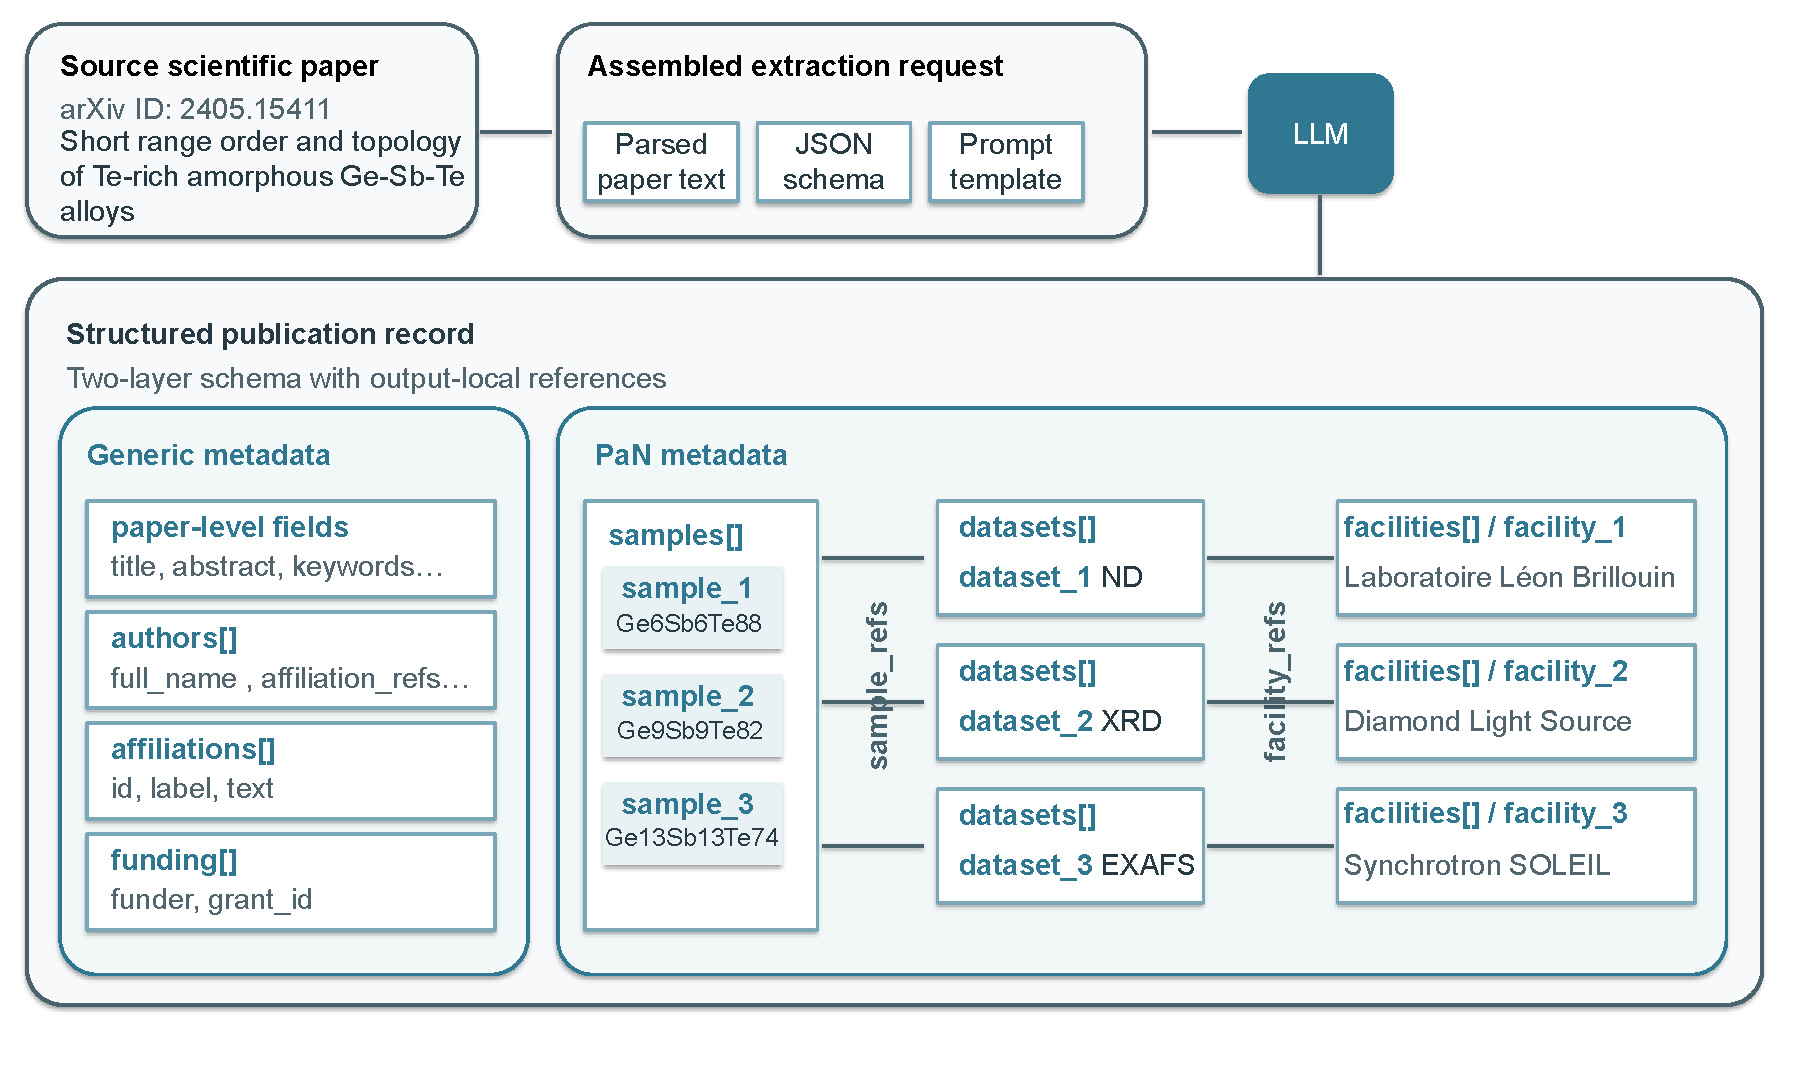
\includegraphics[width=0.95\textwidth]{figures/task_schema.pdf}
  \caption{Task and schema overview. Parsed content from a PaN scientific
  paper is combined with the prompt template and JSON schema to form the
  extraction request supplied to the LLM. The resulting structured publication
  record contains generic and PaN-specific metadata. The example is simplified
  from the reconciled gold record for arXiv:2405.15411, whose three datasets
  each reference the same three samples and one distinct facility. }
  \label{fig:task-schema}
\end{figure*}

\section{PaN Metadata Benchmark}
\label{sec:benchmark}

We formulate publication-derived PaN metadata extraction as the task of
recovering a structured metadata record from a scientific publication according
to a predefined schema. The target combines general publication metadata with
experimental information supported by the publication. We construct a benchmark
of 40 PaN publications for studying this task.

\begin{table}[t]
  \centering
  \small
  \begin{tabular}{@{}lr@{}}
    \toprule
    Item & Count \\
    \midrule
    \multicolumn{2}{@{}l}{\textbf{Corpus and annotation}} \\
    Papers & 40 \\
    Calibration papers & 10 \\
    Evaluation papers & 30 \\
    Working annotations & 90 \\
    \addlinespace
    \multicolumn{2}{@{}l}{\textbf{Repeated entities}} \\
    Affiliations & 179 \\
    Authors & 308 \\
    Funding items & 104 \\
    Facilities & 57 \\
    Samples & 127 \\
    Datasets & 118 \\
    \addlinespace
    \multicolumn{2}{@{}l}{\textbf{Paper-local reference edges}} \\
    Author--affiliation & 354 \\
    Dataset--sample & 321 \\
    Dataset--facility & 73 \\
    \bottomrule
  \end{tabular}
  \caption{Scale of the PaN metadata benchmark. Entity and
  reference counts are derived from the final gold records.}
  \label{tab:benchmark-statistics}
\end{table}


\subsection{Corpus Construction}
\label{sec:corpus}

The benchmark papers were selected from an initial pool of 116
publications retrieved through the arXiv API using technique-oriented search
queries. Selection was designed to cover a broad range of PaN experimental
techniques. Candidate papers were grouped to guide selection across 
small-angle scattering, diffraction, spectroscopy, imaging and tomography, 
reflectometry, and multi-technique studies, together with papers containing 
relatively sparse methodological detail. The resulting 40-paper corpus spans
varied experimental and reporting settings.

\subsection{Structured Metadata Schema}
\label{sec:task-schema}

We define the target metadata through two complementary schema layers. 
The generic schema is intended for reuse across scientific domains and 
captures publication identity and provenance, authors and affiliations, 
funding, and high-level document structure. The PaN schema represents 
experimental facilities, samples, and measurement datasets.

We select and adapt PaN fields from the DAPHNE4NFDI recommendations for 
experiment-time metadata capture \citep{lohstroh2025daphne}, retaining fields 
that can plausibly be supported by scientific publications. The PaN layer 
covers facility information, sample identity and characteristics, and 
dataset-level measurement information such as techniques, acquisition modes, 
and purposes. Together, the two layers define 15 paper-level fields and 
six entity collections, each allowing multiple structured entity records: 
affiliations, authors, funding items, facilities, samples, and datasets.

Each field specifies its semantics, value type, and applicable cardinality 
and structural constraints. Detailed field instructions define inclusion, 
normalization, and entity granularity.

Authors reference affiliations, and datasets reference samples and facilities 
through output-local identifiers such as \texttt{sample\_1} and \texttt{facility\_2}. 
These identifiers allow entities to be referenced by multiple records within an 
output. Their literal values are not globally stable scientific identifiers.

Figure~\ref{fig:task-schema} illustrates this structure using a simplified
excerpt from one reconciled gold record. The complete schema and detailed
field instructions are provided with the benchmark release.

\subsection{Annotation and Gold Construction}
\label{sec:annotation-gold}

Annotation was performed by three annotators. The 40-paper benchmark was 
divided into 10 calibration papers and a 30-paper evaluation set.

During calibration, all three annotators independently annotated the same
10 papers. Comparing these annotations exposed ambiguities in field inclusion,
normalization, entity granularity, and cross-entity references. These cases
were used to refine the schema, field instructions, and annotation protocol
before the evaluation papers were annotated.

The 30-paper evaluation set was divided into three 10-paper batches, with each
batch assigned to a different pair of annotators. Each annotator therefore
completed two batches, and every evaluation paper received two independent 
annotations. Together with the calibration annotations, this produced 90 working 
annotations.

Gold records were produced through reconciliation of the independent
annotations. For each evaluation batch, one annotator resolved disagreements
paper by paper against the source PDFs, and the second annotator reviewed the
resulting records. Reconciliation and review roles were rotated such that each
annotator served as reconciler for one batch and reviewer for another.
Calibration-paper disagreements were similarly resolved against the source
PDFs after protocol refinement. All reconciled records were expressed under
the final schema.

Table~\ref{tab:benchmark-statistics} summarizes the resulting benchmark. The 40
gold records contain 893 entity instances and 748 paper-local
references. In particular, 118 datasets are connected to samples through
321 dataset--sample references, reflecting that one dataset may involve
multiple samples and that one sample may be referenced by multiple datasets.

\section{Entity-Aware Evaluation}
\label{sec:evaluation}

\subsection{Evaluation Framework}
\label{sec:evaluation-framework}

Evaluation follows the structure and semantics of the target schema. Different
metadata fields require different evaluation metrics: constrained values use
exact or normalized-exact match, free text and wording-sensitive names use
ROUGE-L, and unordered lists use set F1. The metric columns in
Tables~\ref{tab:appendix-iaa} and~\ref{tab:appendix-zero-shot} identify the
metric applied to every scored schema field.

Paper-level fields can be evaluated directly against their gold values,
whereas entity collections first require correspondence between
predicted and gold entities. Our evaluation therefore separates three
outcomes: entity recovery, attribute quality among aligned entities, and
reference quality among aligned entities. Because these outcomes
have different meanings and supports, we report them separately rather than
constructing a schema-wide average.


\subsection{Entity Alignment}
\label{sec:entity-alignment}

The six entity collections require one-to-one alignment:
affiliations, authors, funding, facilities, samples, and datasets.

For authors and affiliations, each record provides a direct textual alignment
key: \texttt{full\_name} for authors and \texttt{text} for affiliations.
After normalization, predicted--gold pairs with token-overlap F1 of at least
0.5 are considered candidate matches. Hungarian assignment then selects a
one-to-one matching that maximizes the number of correspondences, with total
similarity used to break ties.

Facilities, funding, samples, and datasets require collection-specific
alignment because their identifying fields can vary in wording and because
similar records may correspond to distinct entities rather than the same one.
For these collections, the evaluator uses the following fields as the primary
basis for alignment: facility \texttt{name}; funding \texttt{grant\_id} and
\texttt{funder}; sample \texttt{sample\_name} and
\texttt{chemical\_composition}; and dataset \texttt{dataset\_name} and
\texttt{measurement\_technique}. Where necessary, these fields are
supplemented with reviewed alternative forms grounded in the source PDF and
entity distinctions recorded during reconciliation. Alternative forms allow
different wording to denote the same entity, whereas entity distinctions
prevent related but separate records from being collapsed. The original field
values are retained for subsequent attribute scoring.

The matching criteria are applied in collection-specific stages. Facilities
are matched by exact name, then by reviewed alternative names for the same
facility, and then by unambiguous complete name containment. For example,
``ESRF'' can correspond to ``European Synchrotron Radiation Facility'' when
the paper defines the acronym, whereas an instrument or beamline named without 
its host facility does not match the facility. Funding records are matched
primarily by normalized grant identifier, with funder information used to 
distinguish records where needed.

Samples are aligned by their names and compositions in the same staged way: first an exact
sample-name match; then a composition that matches and uniquely identifies a
gold sample within the paper; then, among samples of the same composition, 
a match based on distinguishing name words, such as ``with'' sonication versus 
``without'' sonication, or explicit values such as temperature, thickness, or concentration; 
finally, remaining samples are matched when one name contains all words
of the other, as in ``MnSi'' and ``MnSi single crystal'', unless their
reported compositions disagree or another gold sample is an equally
supported match. 

Datasets are aligned similarly using their names and measurement techniques: 
first by the same name with a compatible measurement technique; then by a name that uniquely 
identifies a gold dataset within the paper; then, among datasets sharing a technique, by 
distinguishing words in their names; and finally by technique alone, when the technique identifies 
a single gold dataset and matches only one remaining eligible prediction.

Within each collection, later stages are applied only to entities left
unmatched by earlier stages. Matches follow the collection-specific
criteria above and preserve one-to-one correspondence.

\subsection{Scoring and Aggregation}
\label{sec:scoring-aggregation}

Paper-level fields are scored directly against their gold values using the
field-specific metrics listed in Tables~\ref{tab:appendix-iaa}
and~\ref{tab:appendix-zero-shot}. Scalar paper-level scores are averaged
across papers, while count-based paper-level F1 metrics are micro-aggregated
by pooling true positives, false positives, and false negatives before
computing F1. Section-heading content is scored with set F1; the relative order
of headings is reported only as an appendix diagnostic using Kendall's
$\tau$.

For entity collections, the one-to-one alignment
(Section~\ref{sec:entity-alignment}) determines entity recovery. Aligned
predicted--gold pairs count as true positives, unmatched predictions as false
positives, and unmatched gold entities as false negatives. Entity F1 is
micro-aggregated across the corpus by pooling these counts before computing
F1, so entity-dense papers contribute proportionally.

Attribute metrics are applied only to aligned entity pairs and therefore
measure attribute quality conditional on entity recovery. Scalar attribute
scores are averaged over aligned pairs, while count-based attribute F1 metrics
are micro-aggregated by pooling counts across aligned pairs and papers. Because
the aligned set depends on recovery, conditional attribute scores should be
interpreted together with the corresponding collection's entity F1.

Cross-entity references are scored after predicted output-local identifiers
are remapped through the established entity alignments. For example, if
predicted \texttt{sample\_7} aligns with gold \texttt{sample\_2}, a reference
to \texttt{sample\_7} is evaluated as a reference to
\texttt{sample\_2}. Reference F1 is micro-aggregated across the corpus by
pooling reference true positives, false positives, and false negatives over
aligned parent entities. Reference F1 is therefore conditional and should be
interpreted together with the corresponding parent collection's entity F1.

\section{Experiments}
\label{sec:experiments}

\subsection{Experimental Setup}
\label{sec:experimental-setup}

Table~\ref{tab:experimental-matrix} summarizes the seven evaluated models and
prompting conditions. GPT-5.5 and GPT-4o provide proprietary API-served
reference points, while Mistral Large 3, Gemma 4, and Qwen3.5 provide coverage
of three open-weight model families
\citep{openai2026gpt55,openai2024gpt4o,mistral2025mistral3,
gemmateam2026gemma4,qwenteam2026qwen35}.
The Qwen3.5 4B, 9B, and 27B models form the only within-family size series.

\begin{table*}[t]
  \centering
  \small
  \setlength{\tabcolsep}{6pt}
  \begin{tabular}{@{}p{0.26\textwidth}p{0.26\textwidth}ccc@{}}
    \toprule
    & & \multicolumn{2}{c}{Zero-shot} & Few-shot \\
    \cmidrule(lr){3-4}
    Model snapshot & Access / serving & Full & No inst. & Shots \\
    \midrule
    GPT-5.5 (2026-04-23) & Proprietary; gateway & \checkmark & \checkmark & 1, 3 \\
    GPT-4o (2024-11-20) & Proprietary; gateway & \checkmark & \checkmark & --- \\
    Mistral Large 3 (2512) & Open-weight; gateway & \checkmark & \checkmark & --- \\
    Gemma 4 31B IT & Open-weight; local vLLM & \checkmark & \checkmark & --- \\
    Qwen3.5 27B & Open-weight; local vLLM & \checkmark & \checkmark & 1, 3 \\
    Qwen3.5 9B & Open-weight; local vLLM & \checkmark & \checkmark & 1, 3 \\
    Qwen3.5 4B & Open-weight; local vLLM & \checkmark & \checkmark & 1, 3 \\
    \bottomrule
  \end{tabular}
  \caption{Model and condition coverage. All seven snapshots are run
  zero-shot under both the full-instruction and no-instruction variants;
  four are additionally run with fixed one- and three-example prompts
  with full field instructions. In the reported evaluation, all 22 conditions
  are scored on the same 30 evaluation papers, yielding 660 paper-level
  extractions.}
  \label{tab:experimental-matrix}
\end{table*}


We use zero-shot extraction with the designed generic and PaN schemas,
including their detailed field instructions, as the baseline setting. To
assess the contribution of these instructions, we compare against an
ablation in which the per-field \texttt{instructions} arrays are removed.
We further examine whether examples provide additional benefit by
evaluating one-shot and three-shot prompting for GPT-5.5 and the three
Qwen3.5 models, using fixed demonstrations drawn from the calibration set.

All conditions use a common text-to-JSON extraction pipeline. PDFs are
converted to Markdown-like text with \texttt{pymupdf4llm}, and models receive
the extracted document text together with the schemas and a common extraction
template. Detailed pipeline and serving settings are reported in
Appendix~\ref{app:reproducibility}.

\subsection{Annotation Agreement}
\label{sec:annotation-agreement}

We measure agreement between two independent annotations of each of the 30
evaluation papers using the entity-aware protocol from
Section~\ref{sec:evaluation}. For funding, samples, and datasets, correspondence 
is established through reconciled gold identities. Entity F1 is symmetric under 
annotator-role reversal. Table~\ref{tab:iaa-recovery} reports entity-level agreement 
for the six entity collections. Agreement is perfect for authors and affiliations, 
whose identities  have direct textual anchors in the publication, and remains high 
but imperfect for funding. Agreement is lower for facilities, samples, and datasets, 
where  annotators must additionally decide whether different mentions, states, or 
measurements constitute the same entity or distinct entities.

\begin{table}[t]
  \centering
  \small
  \begin{tabular}{@{}lrrr@{}}
    \toprule
    Entity collection & F1 & Matched & Unmatched \\
    \midrule
    Affiliations & 1.000 & 133 & 0 \\
    Authors & 1.000 & 228 & 0 \\
    Funding & 0.889 & 60 & 15 \\
    Facilities & 0.753 & 29 & 19 \\
    Samples & 0.845 & 71 & 26 \\
    Datasets & 0.793 & 69 & 36 \\
    \bottomrule
  \end{tabular}
  \caption{Pairwise agreement on entity recovery outcomes for
  the 30 evaluation papers.}
  \label{tab:iaa-recovery}
\end{table}


Inspection of unmatched entity records helps explain these differences in
agreement. Funding disagreements mainly reflect decisions about 
whether reported sources of support should be included as funding entities. 
For the PaN collections, the dominant differences concern entity granularity:
representing facilities at the host-facility or instrument/beamline level,
distinguishing sample preparations, treatments, or states, and combining
versus splitting related measurements into dataset entities.

Field-level agreement also varies after entity alignment, with particularly
low agreement for free-text sample and dataset descriptions. The complete
profile is reported in Table~\ref{tab:appendix-iaa}.
\begin{table*}[!t]
  \centering
  \small
  \setlength{\tabcolsep}{2.5pt}
  \begin{tabular}{@{}p{0.19\textwidth}rrrrrrr@{}}
    \toprule
    Entity collection & GPT-5.5 & GPT-4o & Mistral & Gemma & Qwen 27B & Qwen 9B & Qwen 4B \\
    \midrule
    Affiliations & 1.000 & 1.000 & 1.000 & 1.000 & 1.000 & 1.000 & 1.000 \\
    Authors & 1.000 & 1.000 & 1.000 & 1.000 & 1.000 & 1.000 & 1.000 \\
    Funding & 0.954 & 0.925 & 0.912 & 0.945 & 0.953 & 0.901 & 0.810 \\
    Facilities & 0.545 & 0.892 & 0.735 & 0.860 & 0.769 & 0.783 & 0.744 \\
    Samples & 0.800 & 0.777 & 0.865 & 0.864 & 0.837 & 0.783 & 0.739 \\
    Datasets & 0.832 & 0.609 & 0.656 & 0.778 & 0.814 & 0.732 & 0.636 \\
    \bottomrule
  \end{tabular}
  \caption{Full-instruction zero-shot entity recovery for the six
  entity collections on the 30 evaluation papers. All values
  are entity F1.}
  \label{tab:zero-shot-recovery}
\end{table*}

\begin{table*}[!t]
  \centering
  \small
  \setlength{\tabcolsep}{4pt}
  \begin{tabular}{@{}p{0.18\textwidth}rrrrrrr@{}}
    \toprule
    Entity collection & GPT-5.5 & GPT-4o & Mistral & Gemma & Qwen 27B & Qwen 9B & Qwen 4B \\
    \midrule
    Affiliations & +0.000 & +0.000 & +0.000 & +0.000 & +0.000 & +0.000 & +0.000 \\
    Authors & +0.000 & +0.000 & +0.000 & +0.000 & +0.000 & +0.000 & +0.000 \\
    Funding & +0.000 & +0.007 & +0.029 & +0.000 & -0.008 & +0.030 & -0.047 \\
    Facilities & -0.152 & -0.020 & -0.049 & -0.055 & +0.052 & +0.116 & +0.154 \\
    Samples & +0.079 & +0.177 & +0.046 & +0.045 & +0.042 & +0.022 & +0.055 \\
    Datasets & +0.074 & +0.209 & +0.164 & +0.124 & +0.259 & +0.212 & +0.082 \\
    \bottomrule
  \end{tabular}
  \caption{Effect of detailed field instructions on entity recovery
  for the six entity collections on the 30 evaluation papers,
  reported as full-instruction minus no-instruction entity F1.
  Positive values favor the full instructions.}
  \label{tab:instruction-effects}
\end{table*}


\subsection{Baseline Results}
\label{sec:baseline-results}

Table~\ref{tab:zero-shot-recovery} reports entity recovery for the seven
full-instruction zero-shot conditions.
Generic metadata are generally extracted consistently across models: author and
affiliation entity recovery is 1.000 for every model, while title, abstract,
author-name, and affiliation-label scores are all close to one
(Table~\ref{tab:appendix-zero-shot}). Funding entity recovery also remains
comparatively strong, although its attribute scores are less uniform. In
contrast, PaN entity recovery is lower and more variable across facilities,
samples, and datasets.

This contrast may partly reflect how the target metadata are represented in
the publication. Titles, abstracts, authors, and affiliations are typically
localized and explicitly delimited, making their extraction closer to
transcription. Funding has distinctive lexical anchors such as grant
identifiers, but still requires decisions about inclusion and funder--grant
attribution. Facilities, samples, and datasets often require entities to
be constructed from distributed mentions, including decisions about facility
hierarchy, prepared sample variants, and distinct measurement campaigns.
Similar identity and granularity decisions also account for many of the
annotation disagreements observed in
Section~\ref{sec:annotation-agreement}. 

Within the PaN layer, relative model performance depends on the entity type.
GPT-4o achieves the highest facility recovery, while the leading
sample results for Mistral and Gemma are close, and GPT-5.5
achieves the highest dataset recovery. Within the Qwen3.5 series, recovery
increases from 4B to 9B to 27B for samples and datasets, whereas facility 
recovery peaks at 9B. This suggests that the association between model size 
and recovery depends on the entity type rather than following a uniform pattern 
across PaN extraction.

Higher entity recovery does not necessarily correspond to higher quality on
aligned entities. Table~\ref{tab:appendix-zero-shot} reports the corresponding
conditional attribute and reference scores. GPT-4o has the highest facility
entity F1 but the lowest aligned facility-name score (0.747). A stronger
contrast appears for datasets: GPT-5.5 has the highest dataset recovery but,
among its aligned datasets, the lowest dataset--facility reference F1 (0.500),
whereas GPT-4o has substantially lower dataset recovery (0.609) but the highest
conditional dataset--facility reference F1 (0.909). These results show
that entity recovery and conditional attribute and reference quality capture
different aspects of model performance, although the conditional scores are 
computed on model-specific aligned subsets and reference scores additionally 
depend on recovery of the referenced entities.

\begin{figure*}[!t]
  \centering
  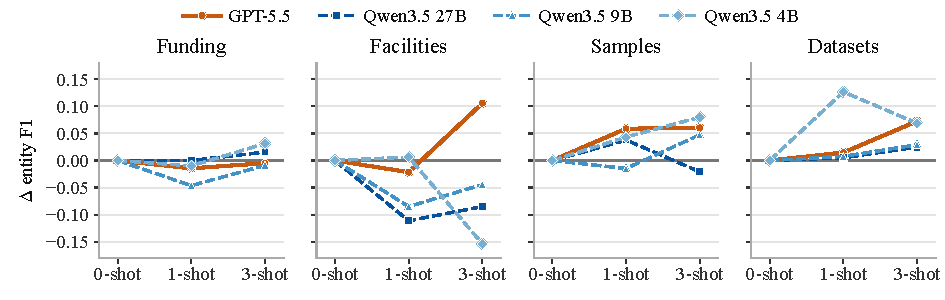
\includegraphics[width=\textwidth]{figures/few_shot.pdf}
  \caption{Effect of fixed demonstrations on entity recovery for the four
  tested models on the 30 evaluation papers, shown as the change in entity F1
  relative to each model's own zero-shot condition (positive values indicate
  higher recovery with demonstrations). Entity F1 for authors and affiliations
  is 1.000 in every condition, so these collections are omitted.}
  \label{fig:few-shot}
\end{figure*}

\subsection{Instruction Ablation}
\label{sec:instruction-ablation}

Table~\ref{tab:instruction-effects} reports the difference in entity F1
between the full-instruction and no-instruction conditions. Detailed instructions
consistently yield higher measured recovery for samples and datasets: dataset
F1 increases by 0.074--0.259 across all seven models, and sample F1 by
0.022--0.177. Author and affiliation recovery is 1.000 with and without
instructions and is therefore unaffected, while funding changes little and in
both directions ($-0.047$ to $+0.030$). Facility recovery shows a different
pattern: instructions reduce F1 for GPT-5.5, GPT-4o, Mistral, and Gemma, but
increase it for all three Qwen3.5 models.

The dataset gains reflect higher recall for six models and
fewer false positives for five. With instructions, six models gain 3--23
dataset true positives; GPT-5.5 retains the same number of true positives and
reduces false positives by 17. False positives are unchanged for Gemma and
increase by one for GPT-4o.

Paired-output inspection suggests that the facility differences partly reflect
how each model's naming and selection behavior interacts with the benchmark's
facility--instrument boundary. The facility instruction requests the specific
facility rather than an umbrella institution, for example PETRA III rather
than DESY, but does not explicitly define the boundary between facilities and
their subordinate instruments or beamlines. For GPT-5.5, Mistral, and Gemma,
instructed outputs often retain an instrument or beamline while omitting the
facility-level name used in the reconciled gold, resulting in fewer recovered
facilities. GPT-4o loses no gold-facility matches; its small F1 decrease comes
from gaining one true positive but three false positives. For all three
Qwen3.5 models, false positives decrease, although their true-positive changes
differ by model. Because the ablation removes the complete instruction bundle
and uses one extraction per paper, these patterns are post hoc explanations
rather than effects isolated to an individual instruction.

\subsection{Few-Shot Demonstrations}
\label{sec:few-shot}

Figure~\ref{fig:few-shot} compares zero-, one-, and three-shot conditions for
GPT-5.5 and the three Qwen3.5 models. Dataset
recovery shows the most consistent three-shot improvement: relative to
zero-shot, entity F1 increases for all four models by 0.025--0.072. Sample
recovery also increases for three of the four models, whereas facility recovery
varies across models and shot counts.

Recovery does not improve monotonically with additional demonstrations.
One-shot and three-shot conditions can move recovery in different directions,
with no consistent ordering across entity types or models. For example,
Qwen3.5 4B dataset F1 rises from 0.636 in zero-shot to 0.763 in one-shot before
decreasing to 0.705 in three-shot, while its sample F1 increases from 0.739 to
0.782 and 0.819. Because only one fixed, ordered set of demonstrations was tested, 
these comparisons characterize the tested prompt configurations and do not isolate 
shot count from exemplar choice.

\FloatBarrier
\section{Conclusion}
\label{sec:conclusion}

We introduced a publication-derived benchmark of 40 PaN papers, with reconciled 
gold records and a two-layer schema for generic and experimental metadata. 
Its entity-aware evaluation aligns entities and remaps output-local identifiers, 
separating entity recovery from conditional attribute and reference quality.

Both annotators and models generally recover paper-level fields, authors,
and affiliations more consistently than facilities, samples, and datasets. 
PaN annotation disagreements frequently concern entity identity and granularity. 
No model leads all three PaN collections, and higher entity recovery does not 
necessarily imply higher conditional attribute or reference quality. Detailed field 
instructions improve dataset and sample recovery across all evaluated models, but 
their effects on facilities are model-dependent. Within the Qwen3.5 family, the 
association between model size and entity recovery depends on the entity
type, while fixed demonstrations produce heterogeneous and sometimes
non-monotonic changes. Together, these findings motivate reporting entity
recovery, attribute quality, and reference quality separately instead of
collapsing them into a benchmark-wide score.

We release the schema, gold records, scoring protocol, and evaluation code to 
support further study of these distinct extraction challenges.

\section*{Limitations}
\label{sec:limitations}

\textbf{Benchmark scope.}
The benchmark is designed for diagnostic coverage rather than statistical
representativeness. Its 40 papers were purposively selected from arXiv to span
diverse PaN techniques and reporting practices, so the observed difficulty
patterns and model results should be interpreted in the context of this
benchmark rather than as representative estimates of performance across PaN
literature.

\textbf{Entity representation.}
The gold records adopt a single set of conventions for entity identity and
granularity. When the publication permits more than one reasonable
representation, such as different facility levels or different groupings of
measurements into datasets, scores reflect both whether a system finds the
relevant information and whether it organizes that information according to
the benchmark's entity boundaries.

\textbf{Alignment generalizability.}
The entity-alignment protocol is benchmark-specific. Its identity criteria
and accepted forms were developed from gold records, source PDFs,
annotation disagreements, and inspection of unmatched model outputs.
Added paper-specific forms require support from the source publication
and gold records, but this does not eliminate the risk of adapting the
protocol to the evaluated outputs. Its applicability to other corpora
or schemas has not been evaluated.

\textbf{Experimental scope.}
Each condition uses one extraction per paper, so the reported values are
single-run point estimates and do not characterize run-to-run generation
variability. The few-shot analysis uses one fixed set of demonstrations,
so differences between shot conditions cannot be attributed to the number
of demonstrations independently of exemplar choice.

\textbf{Input representation.}
All model conditions operate on parsed document text rather than page images,
and some layout-dependent information can be lost during parsing. A targeted
audit found cases in which arXiv identifiers, publication dates, and venue
information printed in rotated margin text were discarded by the parser while
remaining accessible to annotators inspecting the PDFs. Performance on such
fields can therefore partly reflect differences in input access rather than
extraction ability.


\bibliography{custom}

\appendix
\section{Benchmark Corpus}
\label{app:corpus}

The benchmark comprises the 40 photon and neutron science papers listed below,
ordered by arXiv identifier. Each entry links to the public arXiv record.

\begin{small}
\begin{enumerate}\setlength{\itemsep}{1pt}
  \item \href{https://arxiv.org/abs/1804.07163}{arXiv:1804.07163}: Insights into the interactions among Surfactin, betaines, and PAM: surface tension, small-angle neutron scattering, and small-angle X-ray scattering study
  \item \href{https://arxiv.org/abs/1806.08116}{arXiv:1806.08116}: The structure of near stoichiometric Ge-Ga-Sb-S glasses: a reverse Monte Carlo study
  \item \href{https://arxiv.org/abs/1811.10341}{arXiv:1811.10341}: Local order in binary Ge-Te glasses - an experimental study
  \item \href{https://arxiv.org/abs/1812.03956}{arXiv:1812.03956}: X-ray reflectivity with a twist: quantitative time-resolved X-ray reflectivity using monochromatic synchrotron radiation
  \item \href{https://arxiv.org/abs/1901.08819}{arXiv:1901.08819}: Polarized neutron reflectometry study from iron oxide nanoparticles monolayer
  \item \href{https://arxiv.org/abs/1907.00342}{arXiv:1907.00342}: The X-ray photoemission and Co K -Edge X-ray absorption of Ba2CoWO6
  \item \href{https://arxiv.org/abs/1909.08292}{arXiv:1909.08292}: Neutron diffraction and magnetic properties of Co$_2$Cr$_{1-x}$Ti$_x$Al Heusler alloys
  \item \href{https://arxiv.org/abs/1912.11816}{arXiv:1912.11816}: Experimental observation of third-order effect in magnetic small-angle neutron scattering
  \item \href{https://arxiv.org/abs/2001.00707}{arXiv:2001.00707}: Neutron diffraction and ab initio studies on the fully compensated ferrimagnetic characteristics of Mn2V1-xCoxGa Heusler alloys
  \item \href{https://arxiv.org/abs/2001.02706}{arXiv:2001.02706}: Magnetic correlations in the disordered ferromagnetic alloy Ni-V revealed with small angle neutron scattering
  \item \href{https://arxiv.org/abs/2005.01985}{arXiv:2005.01985}: Mechanism of pressure induced amorphization of SnI4: a combined X-ray diffraction -- X-ray absorption spectroscopy study
  \item \href{https://arxiv.org/abs/2006.12074}{arXiv:2006.12074}: Magnetic excitations of Sr$_3$Ir$_2$O$_7$ observed by inelastic neutron scattering measurement
  \item \href{https://arxiv.org/abs/2007.00972}{arXiv:2007.00972}: Synthesis and Characterization of Strontium Doped Barium Titanates using Neutron Diffraction Technique
  \item \href{https://arxiv.org/abs/2009.01093}{arXiv:2009.01093}: X-ray linear dichroic ptychography
  \item \href{https://arxiv.org/abs/2009.12925}{arXiv:2009.12925}: Dynamical spin susceptibility in La2CuO4 studied by resonant inelastic x-ray scattering
  \item \href{https://arxiv.org/abs/2010.00094}{arXiv:2010.00094}: Local and electronic structure of Sr1-xGdxTiO3 probed by X-ray absorption spectroscopy
  \item \href{https://arxiv.org/abs/2010.02965}{arXiv:2010.02965}: New insights into the mechanism of graphene oxide and radionuclide interaction through vacancy defects
  \item \href{https://arxiv.org/abs/2010.12832}{arXiv:2010.12832}: X-ray tomography investigation of cyclically sheared granular materials
  \item \href{https://arxiv.org/abs/2011.13326}{arXiv:2011.13326}: In-situ investigation of temperature induced agglomeration in non-polar magnetic nanoparticle dispersions by small angle X-ray scattering
  \item \href{https://arxiv.org/abs/2104.10884}{arXiv:2104.10884}: X-ray Absorption Spectroscopy Study of La$_{1-y}$Sr$_{y}$Co$_{1-x}$Nb$_x$O$_3$
  \item \href{https://arxiv.org/abs/2105.04167}{arXiv:2105.04167}: Role of higher-order effects in spin-misalignment small-angle neutron scattering of high-pressure torsion nickel
  \item \href{https://arxiv.org/abs/2202.11658}{arXiv:2202.11658}: The honeycomb and hyperhoneycomb polymorphs of IrI$_3$
  \item \href{https://arxiv.org/abs/2203.07170}{arXiv:2203.07170}: In situ study of zinc peroxide decomposition to zinc oxide by X-ray absorption spectroscopy and reverse Monte-Carlo simulations
  \item \href{https://arxiv.org/abs/2209.06540}{arXiv:2209.06540}: Short range order and topology of binary Ge-S glasses
  \item \href{https://arxiv.org/abs/2211.06006}{arXiv:2211.06006}: Small-angle neutron scattering of long-wavelength magnetic modulations in reduced sample dimensions
  \item \href{https://arxiv.org/abs/2212.04169}{arXiv:2212.04169}: Structural changes in Ti1-xAlxN coatings during turning: A XANES and EXAFS study of worn tools
  \item \href{https://arxiv.org/abs/2302.02010}{arXiv:2302.02010}: Identifying f-electron symmetries of UTe2 with O-edge resonant inelastic X-ray scattering
  \item \href{https://arxiv.org/abs/2304.08002}{arXiv:2304.08002}: Morphology of buried interfaces in ion-assisted magnetron sputter deposited 11B4C-containing Ni/Ti multilayer neutron optics investigated by grazing incidence small angle scattering
  \item \href{https://arxiv.org/abs/2309.13729}{arXiv:2309.13729}: Approaching Ferrite-Based Exchange-Coupled Nanocomposites as Permanent Magnets
  \item \href{https://arxiv.org/abs/2404.06853}{arXiv:2404.06853}: Revealing mechanism of pore defect formation in laser directed energy deposition of aluminum alloy via in-situ synchrotron X-ray imaging
  \item \href{https://arxiv.org/abs/2405.14324}{arXiv:2405.14324}: Magnetic microstructure of nanocrystalline Fe-Nb-B alloys as seen by small-angle neutron and X-ray scattering
  \item \href{https://arxiv.org/abs/2405.15411}{arXiv:2405.15411}: Short range order and topology of Te-rich amorphous Ge-Sb-Te alloys
  \item \href{https://arxiv.org/abs/2407.10282}{arXiv:2407.10282}: High-speed synchrotron X-ray imaging of melt pool dynamics during ultrasonic melt processing of Al6061
  \item \href{https://arxiv.org/abs/2407.20626}{arXiv:2407.20626}: Electronic structure and resonant inelastic x-ray scattering in Ta2NiSe5
  \item \href{https://arxiv.org/abs/2410.00268}{arXiv:2410.00268}: Operando Ultrafast Damage-free Diffraction-Enhanced X-ray Absorption Spectroscopy for Chemical Reactivity of Polymer in Solvents
  \item \href{https://arxiv.org/abs/2501.08122}{arXiv:2501.08122}: Origin of perpendicular magnetic anisotropy in ultra-thin metal films studied by in-situ neutron reflectometry
  \item \href{https://arxiv.org/abs/2503.18475}{arXiv:2503.18475}: Rietveld Refinement and NMR Crystallographic Investigations of Multicomponent Crystals Containing Alkali Metal Chlorides and Urea
  \item \href{https://arxiv.org/abs/2601.16215}{arXiv:2601.16215}: High-resolution neutron diffraction determination of noncollinear antiferromagnetic order in the honeycomb magnetoelectric Fe$_{4}$Nb$_{2}$O$_{9}$
  \item \href{https://arxiv.org/abs/2603.01364}{arXiv:2603.01364}: Probing Coordination Environments in Buried Oxides of Aluminum Josephson Junctions by Resonant X-ray Reflectivity
  \item \href{https://arxiv.org/abs/2605.14792}{arXiv:2605.14792}: Thermal expansion of FeWO$_4$ (Ferberite) and FeWO$_4$:Fe$_2$WO$_6$ (7:1): a comparative X-ray and neutron diffraction study
\end{enumerate}
\end{small}


\section{Schema}
\label{app:schema}

The extraction target is defined by a two-layer schema: a generic layer and a PaN
layer. Every field carries a description and a type; top-level fields also declare
a cardinality, and most fields carry an \texttt{instructions} array defining inclusion,
normalization, or entity-granularity decisions. Repeated entities define an
\texttt{item\_schema} for their subfields. Figure~\ref{fig:schema-excerpt} shows
two representative excerpts: the paper-level \texttt{title} field and the
\texttt{samples} entity. The complete set of \emph{scored} fields is enumerated
in the field-level results (Tables~\ref{tab:appendix-iaa} and~\ref{tab:appendix-zero-shot});
the full per-field definitions appear only in the released schema. The no-instruction
variants used in the instruction ablation (Section~\ref{sec:instruction-ablation}) simply
remove the \texttt{instructions} arrays.

\begin{figure*}[t]
\textbf{Paper-level field} (\texttt{bibliographic.title}):
\begin{lstlisting}[style=codeblock]
{
  "title": {
    "description": "Main title of the scientific document itself.",
    "type": "string|null",
    "cardinality": {
      "min": 0,
      "max": 1
    },
    "instructions": [
      "Copy the document title verbatim as printed on the first page or running header. Preserve casing and punctuation."
    ]
  }
}
\end{lstlisting}
\textbf{Entity with sub-schema} (\texttt{samples}, abridged):
\begin{lstlisting}[style=codeblock]
{
  "samples": {
    "description": "Samples studied through experimental measurements reported or reanalyzed in the document. A sample entry can represent a single specimen or a measured group when only the group is identified by the document.",
    "type": "list[sample]",
    "cardinality": {
      "min": 0,
      "max": 50
    },
    "instructions": [
      "Follow this decision routine to determine sample entries.",
      "..."
    ],
    "item_schema": {
      "id": {
        "type": "string",
        "description": "Stable local sample identifier.",
        "instructions": [
          "Assign IDs in sequence: sample_1, sample_2, sample_3, etc.",
          "..."
        ]
      },
      "sample_name": {
        "type": "string",
        "description": "Name, label, or concise identifying phrase for the sample.",
        "instructions": [
          "Follow this decision routine to extract sample_name.",
          "..."
        ]
      },
      "...": "5 further subfields: sample_description, chemical_composition, sample_state, sample_mass, supplier_or_creator"
    }
  }
}
\end{lstlisting}
  \caption{Two excerpts from the released two-layer schema: a paper-level
  field shown in full, and an entity collection with
  its \texttt{item\_schema} of subfields. Each field carries a
  \texttt{description} and \texttt{type}; top-level fields also declare
  a \texttt{cardinality}, and most fields carry an \texttt{instructions}
  array (removed by the no-instruction ablation of
  Section~\ref{sec:instruction-ablation}). The \texttt{samples} entry is
  abridged: long instruction routines and the remaining subfields are
  elided (marked \texttt{...}), and the complete schema with all
  per-field definitions ships with the benchmark.}
  \label{fig:schema-excerpt}
\end{figure*}


\section{Prompt Template}
\label{app:prompt}

All conditions use a single text-to-JSON prompt. The document is converted to
Markdown-like text and inserted together with the schema and an output
skeleton; the model returns one JSON object. Figure~\ref{fig:prompt-template}
shows the zero-shot template.

\begin{figure*}[t]
\begin{lstlisting}[style=codeblock,basicstyle=\ttfamily\scriptsize]
## Task
You are an expert system for extracting metadata from scientific documents.

Extract metadata from the document according to the provided schema.

## Schema

{{SCHEMA_JSON}}

## Rules

- Use only information explicitly stated in the document; do not infer or guess missing information.
- Extract metadata only for the document itself; ignore cited references and other documents mentioned in the text.
- Preserve values exactly as written unless the schema explicitly requires normalization.
- Follow the schema structure strictly.

- For fields with type `string|null`:
  - use a string when the value is present
  - use `null` when the value is not found

- For fields with list types:
  - use a list of extracted items when present
  - use `[]` when no items are found

- For fields with type `boolean`:
  - use `true` when clearly supported by the document
  - use `false` when the document explicitly states the contrary

- For nested objects and list items:
  - follow the schema structure exactly
  - fill subfields according to their declared types

## Output Format

Return a single valid JSON object matching the skeleton below exactly.
- Use double-quoted object keys and double-quoted string values.
- Do not wrap the JSON in code fences (```), markdown, or any other formatting.
- Do not add fields not defined in the skeleton.
- Do not omit fields defined in the skeleton.
- Do not return explanations, comments, or natural-language text outside the JSON.

{{OUTPUT_SKELETON}}

## Document

{{DOCUMENT_TEXT}}
\end{lstlisting}
  \caption{Zero-shot extraction prompt template. \texttt{\{\{SCHEMA\_JSON\}\}},
  \texttt{\{\{OUTPUT\_SKELETON\}\}}, and \texttt{\{\{DOCUMENT\_TEXT\}\}} are
  replaced at request time. The few-shot template additionally inserts an
  \texttt{Examples} block of complete worked extractions before the
  document.}
  \label{fig:prompt-template}
\end{figure*}


\section{Reproducibility Details}
\label{app:reproducibility}

All 660 extractions included in the reported evaluation use one text-to-JSON
pipeline under the fixed settings in Table~\ref{tab:setup}. Each of the 22
conditions contains exactly one extraction per target paper, so all reported
scores are single-run point estimates without seed averaging. The seven model
snapshots are pinned to the versions in
Table~\ref{tab:experimental-matrix}.

\begin{table}[t]
  \centering
  \small
  \begin{tabular}{@{}ll@{}}
    \toprule
    Setting & Value \\
    \midrule
    \multicolumn{2}{@{}l}{\textit{Document input}} \\
    PDF-to-text & \texttt{pymupdf4llm} 1.27.2.2 \\
    \addlinespace
    \multicolumn{2}{@{}l}{\textit{Decoding}} \\
    Temperature & 0 \\
    Reasoning / thinking & Disabled \\
    Max output tokens & 12{,}288 \\
    Runs per condition & 1 \\
    \addlinespace
    \multicolumn{2}{@{}l}{\textit{Local serving (Gemma 4, Qwen3.5)}} \\
    Engine & vLLM 0.24.0 \\
    GPU & NVIDIA A100 80GB \\
    \addlinespace
    \multicolumn{2}{@{}l}{\textit{Hosted serving (GPT-5.5, GPT-4o, Mistral)}} \\
    Access & OpenAI-compatible gateway \\
    \bottomrule
  \end{tabular}
  \caption{Fixed pipeline settings applied to all 22 conditions.
  Per-model serving mode and the pinned model
  snapshots are listed in Table~\ref{tab:experimental-matrix}.}
  \label{tab:setup}
\end{table}


The schema, prompt template, reconciled gold records, scoring plan, alignment
helper, and evaluation code are released with the benchmark.


\section{Complete Field-Level Results}
\label{app:complete-results}

This appendix reports the complete field-level evaluation results. Section
headings have separate rows for content recovery and relative order; all other
fields appear once. The metric used for each row is shown in the tables.
Fields with no or very few non-null gold values are flagged
($^{\dagger}$/$^{\ddagger}$). Their scores are reported for completeness but
are not interpreted.

The three F1 variants use the same formula but differ in how matches are
determined: set F1 uses exact matching after normalization, entity F1 uses the
one-to-one alignment described in Section~\ref{sec:entity-alignment}, and
reference F1 is computed after predicted output-local identifiers are remapped
through that alignment.

Table~\ref{tab:appendix-iaa} reports the complete pairwise annotation agreement
results for the 30-paper evaluation set.

\begin{table*}[t]
  \centering
  \footnotesize
  \setlength{\tabcolsep}{6pt}
  \begin{tabular}{@{}p{0.34\textwidth}p{0.18\textwidth}r@{}}
    \toprule
     & Metric & Agreement \\
    \midrule
    \multicolumn{3}{@{}l}{\textit{Paper-level fields}} \\
    Title & ROUGE-L & 0.957 \\
    Subtitle$^{\dagger}$ & ROUGE-L & 1.000 \\
    Abstract & ROUGE-L & 0.996 \\
    DOI$^{\dagger}$ & Normalized exact & 1.000 \\
    arXiv ID & Normalized exact & 1.000 \\
    URL$^{\dagger}$ & Normalized exact & 1.000 \\
    Publication date & Exact & 0.900 \\
    Venue & Normalized exact & 1.000 \\
    Publisher$^{\dagger}$ & Normalized exact & 1.000 \\
    Language & Exact & 1.000 \\
    Keywords & Set F1 & 0.976 \\
    Section-heading content & Set F1 & 0.969 \\
    Section-heading order & Kendall $\tau$ & 1.000 \\
    Has references & Exact & 1.000 \\
    Has figures & Exact & 1.000 \\
    Has tables & Exact & 1.000 \\
    \addlinespace
    \midrule
    \multicolumn{3}{@{}l}{\textit{Affiliations}} \\
    Affiliation entities & Entity F1 & 1.000 \\
    Affiliation label & Normalized exact & 0.962 \\
    Affiliation text & ROUGE-L & 0.997 \\
    \addlinespace
    \midrule
    \multicolumn{3}{@{}l}{\textit{Authors}} \\
    Author entities & Entity F1 & 1.000 \\
    Author full name & Normalized exact & 0.996 \\
    Author ORCID$^{\dagger}$ & Normalized exact & 1.000 \\
    Author email & Normalized exact & 1.000 \\
    Corresponding-author flag & Exact & 0.987 \\
    Author--affiliation refs & Reference F1 & 1.000 \\
    \addlinespace
    \midrule
    \multicolumn{3}{@{}l}{\textit{Funding}} \\
    Funding entities & Entity F1 & 0.889 \\
    Funder & ROUGE-L & 0.837 \\
    Grant ID & Normalized exact & 0.900 \\
    \addlinespace
    \midrule
    \multicolumn{3}{@{}l}{\textit{Facilities}} \\
    Facility entities & Entity F1 & 0.753 \\
    Facility name & ROUGE-L & 0.776 \\
    \addlinespace
    \midrule
    \multicolumn{3}{@{}l}{\textit{Samples}} \\
    Sample entities & Entity F1 & 0.845 \\
    Sample name & ROUGE-L & 0.740 \\
    Chemical composition & Normalized exact & 0.817 \\
    Sample state & Normalized exact & 0.718 \\
    Sample mass$^{\ddagger}$ & Normalized exact & 0.986 \\
    Sample description & ROUGE-L & 0.180 \\
    Supplier / creator & ROUGE-L & 0.845 \\
    \addlinespace
    \midrule
    \multicolumn{3}{@{}l}{\textit{Datasets}} \\
    Dataset entities & Entity F1 & 0.793 \\
    Dataset name & ROUGE-L & 0.693 \\
    Measurement technique & ROUGE-L & 0.864 \\
    Dataset description & ROUGE-L & 0.361 \\
    Measurement mode & Set F1 & 0.700 \\
    Dataset purpose & Exact & 0.957 \\
    Dataset--sample refs & Reference F1 & 0.855 \\
    Dataset--facility refs & Reference F1 & 0.814 \\
    \bottomrule
  \end{tabular}
  \caption{Complete pairwise annotation agreement on the 30
  evaluation papers. Attribute and reference rows are
  conditional on aligned parents. A $^{\dagger}$ marks a field with
  no non-null support and a $^{\ddagger}$ one with at most 10\%
  non-null support.}
  \label{tab:appendix-iaa}
\end{table*}


Table~\ref{tab:appendix-zero-shot} reports the complete field-level results for
all seven models under the full-instruction zero-shot setting on the 30-paper
evaluation set.

Three paper-level fields marked $^{\S}$ are affected by the PDF-to-text
conversion: arXiv ID, publication date, and venue. On affected papers, the
relevant evidence appears only in the rotated first-page arXiv stamp, which
\texttt{pymupdf4llm} omits from the model input. Most notably, the arXiv-ID
score of 0.533 reflects null--null agreement on 16 papers and no successful
recovery on the 14 papers with non-null gold values. Scores for these fields
therefore partly reflect unavailable input evidence rather than model
extraction alone.

\begin{table*}[t]
  \centering
  \fontsize{8.5pt}{9.5pt}\selectfont
  \setlength{\tabcolsep}{2pt}
  \begin{tabular}{@{}p{0.24\textwidth}p{0.13\textwidth}rrrrrrr@{}}
    \toprule
     & Metric & GPT-5.5 & GPT-4o & Mistral & Gemma & Qwen 27B & Qwen 9B & Qwen 4B \\
    \midrule
    \multicolumn{9}{@{}l}{\textit{Paper-level fields}} \\
    Title & ROUGE-L & 0.994 & 0.992 & 0.995 & 0.990 & 0.990 & 0.992 & 0.993 \\
    Subtitle$^{\dagger}$ & ROUGE-L & 0.967 & 0.967 & 1.000 & 1.000 & 1.000 & 1.000 & 1.000 \\
    Abstract & ROUGE-L & 0.976 & 0.987 & 0.982 & 0.973 & 0.974 & 0.980 & 0.977 \\
    DOI$^{\dagger}$ & Normalized exact & 1.000 & 0.967 & 1.000 & 0.967 & 1.000 & 0.967 & 1.000 \\
    arXiv ID$^{\S}$ & Normalized exact & 0.533 & 0.533 & 0.533 & 0.533 & 0.533 & 0.533 & 0.533 \\
    URL$^{\dagger}$ & Normalized exact & 1.000 & 1.000 & 1.000 & 1.000 & 1.000 & 1.000 & 1.000 \\
    Publication date$^{\S}$ & Exact & 0.800 & 0.767 & 0.667 & 0.800 & 0.800 & 0.767 & 0.800 \\
    Venue$^{\S}$ & Normalized exact & 0.567 & 0.567 & 0.600 & 0.567 & 0.567 & 0.567 & 0.667 \\
    Publisher$^{\dagger}$ & Normalized exact & 1.000 & 0.933 & 0.933 & 0.967 & 0.967 & 0.933 & 0.967 \\
    Language & Exact & 1.000 & 1.000 & 1.000 & 1.000 & 1.000 & 0.967 & 1.000 \\
    Keywords & Set F1 & 1.000 & 1.000 & 1.000 & 1.000 & 1.000 & 0.976 & 0.909 \\
    Section-heading content & Set F1 & 0.945 & 0.763 & 0.660 & 0.949 & 0.969 & 0.635 & 0.710 \\
    Section-heading order & Kendall $\tau$ & 1.000 & 1.000 & 1.000 & 1.000 & 1.000 & 1.000 & 1.000 \\
    Has references & Exact & 1.000 & 1.000 & 1.000 & 1.000 & 1.000 & 1.000 & 1.000 \\
    Has figures & Exact & 1.000 & 1.000 & 1.000 & 1.000 & 1.000 & 1.000 & 1.000 \\
    Has tables & Exact & 1.000 & 1.000 & 0.967 & 1.000 & 1.000 & 1.000 & 1.000 \\
    \addlinespace
    \midrule
    \multicolumn{9}{@{}l}{\textit{Affiliations}} \\
    Affiliation entities & Entity F1 & 1.000 & 1.000 & 1.000 & 1.000 & 1.000 & 1.000 & 1.000 \\
    Affiliation label & Normalized exact & 1.000 & 0.977 & 1.000 & 1.000 & 1.000 & 1.000 & 0.970 \\
    Affiliation text & ROUGE-L & 0.999 & 0.997 & 0.999 & 0.999 & 0.999 & 0.999 & 0.999 \\
    \addlinespace
    \midrule
    \multicolumn{9}{@{}l}{\textit{Authors}} \\
    Author entities & Entity F1 & 1.000 & 1.000 & 1.000 & 1.000 & 1.000 & 1.000 & 1.000 \\
    Author full name & Normalized exact & 1.000 & 0.991 & 1.000 & 1.000 & 1.000 & 1.000 & 1.000 \\
    Author ORCID$^{\dagger}$ & Normalized exact & 1.000 & 1.000 & 1.000 & 1.000 & 1.000 & 1.000 & 1.000 \\
    Author email & Normalized exact & 0.996 & 0.996 & 0.996 & 0.996 & 0.996 & 0.991 & 0.978 \\
    Corresponding-author flag & Exact & 0.991 & 0.991 & 1.000 & 0.982 & 1.000 & 0.982 & 0.965 \\
    Author--affiliation refs & Reference F1 & 1.000 & 1.000 & 1.000 & 1.000 & 1.000 & 0.994 & 0.996 \\
    \addlinespace
    \midrule
    \multicolumn{9}{@{}l}{\textit{Funding}} \\
    Funding entities & Entity F1 & 0.954 & 0.925 & 0.912 & 0.945 & 0.953 & 0.901 & 0.810 \\
    Funder & ROUGE-L & 0.872 & 0.833 & 0.822 & 0.892 & 0.885 & 0.829 & 0.818 \\
    Grant ID & Normalized exact & 0.694 & 0.855 & 0.790 & 0.850 & 0.770 & 0.875 & 0.878 \\
    \addlinespace
    \midrule
    \multicolumn{9}{@{}l}{\textit{Facilities}} \\
    Facility entities & Entity F1 & 0.545 & 0.892 & 0.735 & 0.860 & 0.769 & 0.783 & 0.744 \\
    Facility name & ROUGE-L & 0.820 & 0.747 & 0.806 & 0.816 & 0.855 & 0.767 & 0.812 \\
    \addlinespace
    \midrule
    \multicolumn{9}{@{}l}{\textit{Samples}} \\
    Sample entities & Entity F1 & 0.800 & 0.777 & 0.865 & 0.864 & 0.837 & 0.783 & 0.739 \\
    Sample name & ROUGE-L & 0.788 & 0.840 & 0.734 & 0.854 & 0.884 & 0.772 & 0.783 \\
    Chemical composition & Normalized exact & 0.750 & 0.689 & 0.688 & 0.645 & 0.611 & 0.615 & 0.655 \\
    Sample state & Normalized exact & 0.486 & 0.443 & 0.532 & 0.658 & 0.667 & 0.569 & 0.552 \\
    Sample mass$^{\ddagger}$ & Normalized exact & 0.944 & 0.852 & 0.987 & 0.947 & 0.986 & 0.954 & 0.966 \\
    Sample description & ROUGE-L & 0.403 & 0.240 & 0.280 & 0.444 & 0.306 & 0.326 & 0.261 \\
    Supplier / creator & ROUGE-L & 0.846 & 0.790 & 0.675 & 0.781 & 0.847 & 0.747 & 0.738 \\
    \addlinespace
    \midrule
    \multicolumn{9}{@{}l}{\textit{Datasets}} \\
    Dataset entities & Entity F1 & 0.832 & 0.609 & 0.656 & 0.778 & 0.814 & 0.732 & 0.636 \\
    Dataset name & ROUGE-L & 0.717 & 0.576 & 0.723 & 0.722 & 0.732 & 0.702 & 0.510 \\
    Measurement technique & ROUGE-L & 0.747 & 0.903 & 0.871 & 0.886 & 0.950 & 0.863 & 0.839 \\
    Dataset description & ROUGE-L & 0.444 & 0.277 & 0.371 & 0.333 & 0.390 & 0.333 & 0.412 \\
    Measurement mode & Set F1 & 0.752 & 0.475 & 0.463 & 0.590 & 0.681 & 0.333 & 0.495 \\
    Dataset purpose & Exact & 1.000 & 1.000 & 0.984 & 1.000 & 0.958 & 1.000 & 1.000 \\
    Dataset--sample refs & Reference F1 & 0.743 & 0.812 & 0.849 & 0.831 & 0.832 & 0.693 & 0.802 \\
    Dataset--facility refs & Reference F1 & 0.500 & 0.909 & 0.767 & 0.851 & 0.771 & 0.809 & 0.746 \\
    \bottomrule
  \end{tabular}
  \caption{Complete full-instruction zero-shot results on the 30 evaluation
  papers. Paper-level scalar and order scores are averaged
  over papers; scalar entity-attribute scores are averaged over aligned
  pairs; count-based set, entity, and reference F1 scores are
  micro-aggregated across the corpus. Attribute and reference scores are
  conditional
  on aligned parents. A $^{\dagger}$ marks a field
  with no gold non-null values and a $^{\ddagger}$ one with at most
  10\% gold non-null support. A $^{\S}$ marks fields whose gold evidence is
  discarded during PDF-to-text conversion on some papers, as
  detailed in Appendix~\ref{app:complete-results}.}
  \label{tab:appendix-zero-shot}
\end{table*}



\end{document}
